%\section{Motivation}

% - What is the major field i am in?
% - what are the biological questions 
% - how are they typically slved

% - problems with the current solutions


% In much of nature, the idea of size scales is widely discussed and investigated. From a basic understanding of physics, one understands that the forces an object feels are directly linked to their mass or volume and mass density. For example, we can easily understand what will happen to a basketball if we throw it up into the air as we are sitting on planet earth. However, when we leave the familar size scale, such as having a basketball the size of planet earth, or the size of a gas molecule, our intuition begins to show its cracks. 

Objects that exist in nature can be divided into macroscopic and microscopic entities. Macroscopic objects can be directly measured with a ruler or a photograph. However, as microscopic objects become smaller than the wavelength of light, they become un-resolveable by the light alone. Thus, one must resort to other methods to recover their size. 

At the nanoscale, thermal energy, $k_bT$, is comparable to, or larger than the gravitational and inertial energy scales that typical govern macroscopic dynamics. In the case of liquids, the thermal energy emerges into a motion in Reynold's numbers $\Re \ll 1$, where the viscous drag dominates ver the inertia. The result is a stochastic, thermal motion that governs particle transport. 

The relation between the particle's size and its motion is explained in Einstein's seminal paper \cite{einstein1956investigations} where the rate of transport, or diffusion is related to the particle's size,
\begin{equation}
    D(\vec{x}, a) = \frac{k_bT}{\gamma(\vec{x}, a)},
\end{equation}

where $\gamma(\vec{x}, a)$ is the viscous drag at the position $\vec{x}$ of a particle of hydrodynamic radius $a$. In the case of a spherical paricle in an incompressible fluid, $\gamma(a) = 6\pi \eta a$, where $\eta$ is the fluid viscosity. 

In typical measurements of particle motion, it is easiest to work in a confined space. For instance, convex-lens induced confinement (CLiC) measurements typically use micro-apertures of volume $\SI{1.5}{\micro \meter^3}$ to confine single molecules for extended temporal measurements via fluorescence microscopy. This is similar in the case of nanoparticle tracking analysis (NTA) measurements, where a flow is applied to particles confined between two plates in a flow-cell and are imaged using scattering microscopy. The confinement is performed as microscope images consist of 2D slices of a focal plane, which is typically on the order of a few hundred nanometers (cite). 

Although experimentally easier, the viscous drag relation is spatially varying. In turn, size-diffusivity relation in confinement is intrinsically non-trivial. This non-trivial behavior can been shown to alter the diffusivity of a particle by a significant amount \cite{swanParticleMotionParallel2010,bian111YearsBrownian2016}. 

Since the diffusivity of a particle in confinement is spatially varying, in order to recover the true size of a particle diffusing, it is necessary to have the full spatial location of the particle's motion with respect to the confinement barriers. This requirement necessitates the 3D tracking in confinement experiments. If one does not have the 3 dimensional position, one cannot recover the true size estimate.

In addition, one would like to view the molecules for enough frames to collect enough positional information to extrapolate the size. Thus, it would be better to use scattering microscopy over fluorescence as the photobleaching time of fluorescence and SNR is a hinderance to having quality data. 

\begin{figure}[ht]
    \centering
    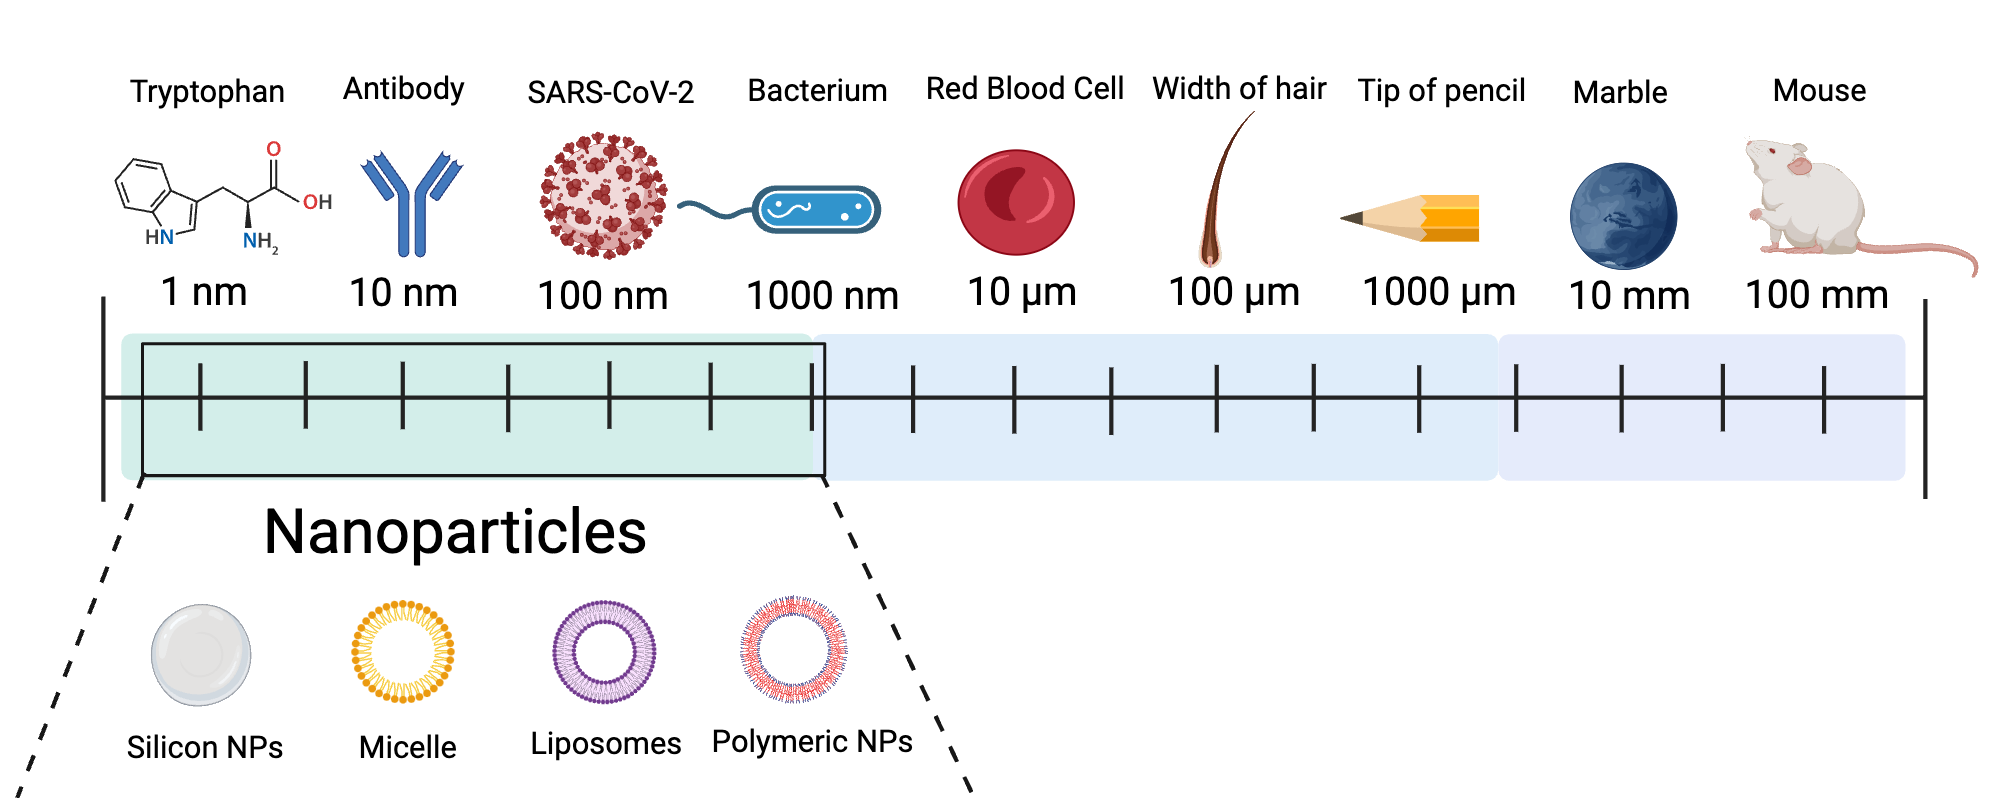
\includegraphics[width=\textwidth]{Figures/size-comp.png}
    \caption{Size comparison of various nanoparticles. Nanoparticles are defined as particles where the largest dimension is at most $\SI{1000}{\nm}$.}
\end{figure}

In the realm of biological processes, there are many such examples involving the particles in the nano size regime. For example, viruses and vesicles are two examples of small molecules which have immense importance in the field. To investigate such systems, it is often the case that to maintain long measurements of the same particle, it is necessary to have some form of confinement. The full understanding of the behavior of these nanoparticles under confinement is thus important, and not complete. 

The thesis consists of 8 chapters. Chapter 2 provides a description of the literature of confined brownian motion over the last century. Chapter 3 describes the theoretical description of interferometric scattering microscopy (iSCAT) and physical limits that apply in optical theory. Chapter 4 discusses the application of Brownian motion and iSCAT in a biological context, which details regarding lipid-nanoparticles and why they need to be studied on the single-molecule level. Chapter 5 consists of investigations of confined diffusion using Langevin simulations. A simulated system was developed and the size-diffusivity relation in an electrostatically screened system was investigated. Chapter 6 describes the 3D iSCAT tracking technique developed during this work. The method overview and validation and explicitly developed and validated Chapter 7 describes the method applied to experimental data and utilizes various nanoparticle species, highlighting their varied diffusions. Chapter 8 concludes the world and provides a future outlook on the topic and steps which need to be advanced.


